\chapter{Software Development at HubSpot}
Software development has been a core part of HubSpot since day one. As such, the overall development process and methodology has undergone several iterations. Critically, at each iteration, the development process is reevaluated and the experience gained over the past number of years is capitalized upon. This has lead to a streamlined and simple development process which is easy to learn, allowing both new hires and temporary interns to get up to speed quickly. HubSpot also has several \textit{platform} teams soley dedicated to providing easy to use integrations of powerful tools which can be combersome to configure on a per project basis. These teams contribute to what's known as a the overall \textit{platform as a service (PaaS)}. Product development teams can then use this platform to get access to these powerful tools, without needing to spend time on configuration.

As all of HubSpot is built on the same technology stack and all projects adhere to a common project structure, any developer can drop into any project owned by another team and immediately know where to search for what they are looking for. This has the direct benefits of allowing engineers to fix bugs they encounter when using other teams' projects. One of HubSpot's core beliefs when it comes to software engineering is that everyone should contribute what they can, instead of passing the blame to other teams. Most engineers are busy with new tasks and challenges and fixing a bug in code that belongs to a fellow engineer is substantially more productive for \textbf{both} teams than filing an issue and waiting for it to be resolved. 

\section{Technologies in use at HubSpot}
As discussed, all of HubSpot is built using a set of technologies. This set of technologies is continuously growing as needs change and as new technologies become available. Typically any given team and/or project will use a subset of the technologies on offer. This section outlines some of the core technologies used by the \team{} team. 
\subsection{Java 8}
Java 8 is the second to newest release of Java. Java as a language has been around since the mid 1990s and has been under continuous development since then. As such, it has become a very stable and reliable language, used by nine million developers world wide \cite{java9Million}. At HubSpot, Java 8 is used for the development of all backend services. The architecture employed is one of micro-services. This allows for rapid development and deployment of many loosely coupled services. The services are extremely modular and are often used by a variety of teams and projects. 

Java is an object oriented language which provides a variety of concepts to aid in system design. Classically, the core of object oriented programming is that entities (objects) should model one \textit{real} entity and one only. Objects can then be used inside of other classes, abstracting away all of the complex implementation logic of the class in use from the user. Any information required by the object can be encapsulated within the object itself allowing the object to provide a simple interface to it's users, coinsisting of a number of methods, which if named correctly, provide a succinct description of what the method does which lines up exactly with what the user thinks the method should do.

Java 8 was released in March of 2014 and provides several new and extremely powerful features, many of which are used on a daily basis at HubSpot. Aside from all of the core functionality contained in Java, a subset of the most interesting and useful features it provides are outlined below.


%% Lambdas
\sneaktitle{Lambda Expressions}
Often times it is useful to create classes which wrap a piece of logic or code. Similarly, systems often require the execution of a piece of code in response to a certain event (e.g. running some code in response to a mouse click). Traditionally in java this was accomplished by writing a manual \textit{functional interface}. There functional interfaces were simple interfaces which provided a contract containing a single method. The class class in question can then be passed an instance of an object which implements the functional interface and can thus invoke the method defined in the interface when appropriate. An example of this using traditional java is outlined in \refcode{lst:noLambda} which contains code for a button that can be clicked and can have on-click methods associated with it. Prior to Java 8, this code was cumbersome to write requiring a custom interface to be created, implemented by a concrete class and its implementation instantiated and passed to the class. 

\lstinputlisting[
  caption={onClick Listener without Lambda Expression},
  label={lst:noLambda},
  style=javaStyle
  ]{code/technologies/NoLambda.java}

This code can be written in a much more concise form by using Java 8's new lambda expressions. The JDK now provides the most common functional interfaces which can be used in place of custom functional interfaces. For example the \java{Consumer<T>} functional interface, defines a single \java{accept} function which takes an argument of type \java{T} and returns nothing (it \textit{consumes} the argument), which is exactly what our \java{OnClickRunner} defined. The \java{Button} class can be refactored to use a \java{Consumer<String>}, allowing the logic of the \java{OnClickRunner} to be directly specified through a lambda expression. An example of this is shown in \refcode{lst:withLambda} and the lambda expression can be seen on line 16.

\lstinputlisting[
  caption={onClick Listener with Lambda Expression},
  label={lst:withLambda},
  style=javaStyle
  ]{code/technologies/Lambda.java}


%% Streams
\sneaktitle{Streams}
Another extremely powerful feature of Java 8 is the new Stream API. This allows for the bulk processing of collections through map/reduce like operations. Performing arbitrary data manipulation on a collection of Java objects is extremely common. Typically this could be accomplished using a simple loop. However this often requires the introduction of several local variables which can add excessive noise to code. Of course, some operations are still better suited to a simple loop, particularly if the data transformation function has side effects, in which case it is impossible to use streams. However it is widely considered good practice to minimize side effects of functions in order to maintain simplicity and making heavy use of streams is a great way to remind developers not to introduce side effects and to in general, minimize the amount of state required by a class. The Java 8 Stream API is fluent, allowing for arbitrarily complex stream operations to be chained together. Streams are also evaluated lazily, minimizing the amount of work to be done and can be parallelized internally by the API, providing excellent performance. The Java 8 Stream API consists of three types of operations: 

\begin{labeling}{Intermediate Operations}
	\item [Initial stream call] The \java{stream()} call can be invoked on any Java collection of objects. This call returns a \java{Stream<T>} where \java{T} is the type of the objects in the collection, allowing subsequent intermediate and terminal operations to be invoked on the returned stream.
	\item [Intermediate Operations] These are the operations which perform the data transformation. There are a variety of intermediate operations provided such as \java{sort} which sorts the objects in the stream, \java{filter} which filters objects in the stream according to some predicate and \java{map} which maps an arbitrary function over each object in the stream. As mentioned, the Stream API is fluent, meaning multiple intermediate operations can be chained together (for example filtering the objects and then sorting them).
	\item [Terminal Operations] The is the final operation which describes how the data should be reduced to a single object (which may be a collection). Common terminal operations are \java{max} which returns the maximum of the objects in the stream, \java{findFirst} which returns the first object the stream encounters that matches a given predicate and \java{collect} which defines how the objects in the stream should be collected into a collection (for example collecting the objects into a set would remove any duplicates)
\end{labeling}

Comparing \refcode{lst:withoutStreams} and \refcode{lst:withStreams}, the clarity of the code produced using the Streams API can be seen. The code shows two approaches to a piece of code which returns the length of each of the strings (in ascending order) without whitespace and which don't contain the word \textit{owl}. Although this is a toy example, several benefits of the Streams API can be seen. The code using streams (\refcode{lst:withStreams}) reads like the steps of an recipie, clearly stating what is performed at each step. However the code using the traditional \java{for} loop (\refcode{lst:withoutStreams}), requires \java{if} statements and redundant local variables, distracting the programmer from the core steps of the algorithm. Streams also provide the benefits of immutability and parallelism for free.

\lstinputlisting[
  caption={Batch Processing without Streams},
  label={lst:withoutStreams},
  style=javaStyle
  ]{code/technologies/NoStreams.java}

\lstinputlisting[
  caption={Batch Processing with Streams},
  label={lst:withStreams},
  style=javaStyle
  ]{code/technologies/Streams.java}


%% Completable Futures
\sneaktitle{Completable Futures}
Asynchronus programming is present in most if not all modern systems. In the early days of Java, this was accomplished by the JDK through abstractions at the thread level. This required careful tracking of the state of threads by the programmer. Concurrent programs are incredibly difficult to reason about and thus concurrency is one of the most challening aspects of modern software engineering and is the source of a huge number of bugs. However the benefits of concurrent programming are extremely obvious, essentially making it a nescesity in modern systems. Thus any abstractions that can aid in reducing the number of things a programmer must keep track of will be beneficial. In Java 8's case, this abstraction is the CompletableFuture API. This API allows for programmers to perform asynchronus tasks by specifying a \java{Supplier<U>}, a function which takes no arguments and returns (supplies) a value of type \java{U}, which will return a value at some point in the future. Thus what's returned from this call is not an instance of type \java{U}, but a \java{CompletableFuture<U>}, that is, an object that at some point in the future will contain an instance of type \java{U} (provided no errors occur). 

The programmer may also specify an \java{Executor} \cite{javaExecutor} which is essentially an object (e.g. threadpool) capable of running tasks on a thread other than the thread in the current context. If no \java{Executor} is specified, the task is automatically submited to Java's work stealing \java{ForkJoinPool} \cite{javaForkJoinPool}. 

The API provides a simple \java{get} method for blocking until the return value is present (or throws an exception). More interestingly however, it also provides several methods to specify subsequent processing of the return value when it returns. A subset of these methods are the following \cite{javaCfArticle}:

\begin{labeling}{thenCompose}
	\item [thenApply] This method is used to supply a function that should be run upon completion of the underlying \java{CompletableFuture}. The result of the \java{CompletableFuture} will be passed as the sole argument to this function. This function is free to return any type and in doing so, sets the type associated with the underlying \java{CompletableFuture}. 
	\item [thenCompose] This method is very similar to \java{thenApply} except it is used when the desired function to be run is also asynchronus (that is, it too returns a completable future). This behaviour could technically also be handled by /java{thenApply} (as it is free to return any value), but this would cause the return type of the parent \java{CompletableFuture} to itself be a \java{CompletableFuture}. The benefit of \java{thenCompose} is that it contains logic to unwrap this nested \java{CompletableFuture}, allowing the return type of the parent to remain a \java{CompletableFuture<T>} even if the supplied function is asynchronus.
	\item [thenAccept] This method is used when the return type of the \java{CompletableFuture} only needs to be used in the registered callback and is not used outside of the supplied function. As such, this method takes a \java{Consumer<T>} as its argument, that is, a function which takes \java{T} as a parameter and does not return anything.  
\end{labeling}


\subsection{Guice - Dependency Injection}\label{sec:guice}
Google's Guice \cite{guice} is a dependency injection framework for Java. Dependency injection is a software pattern which abstracts away the actual construction (instantiation) of objects from the user. As a system grows and abstractions are built atop one and other, simply instantiating an object can be come tedious and difficult. Traditionally, in order to instantiate an object, all of its unconditionally required dependencies must be passed to the constructor of the object. Otherwise the object could be left in an inconsistent state. Thus in order to instantiate an object \java{O}, all of its dependencies, for example \java{X, Y and Z} must be provided to \java{O}'s constructor. Thus the client of \java{O} must first instantiate instances of \java{X, Y and Z} before it can use \java{O}. However \java{X} may have it's own set of dependencies and the problem simply gets worse and worse. An example of the difficulties this can cause (based on the example in Guice's documentation \cite{guiceDocs}) is shown in \refcode{lst:noDI}. The code shown has to recursively create each of the dependencies for each of it's dependencies which can quickly get out of hand for large systems.

\lstinputlisting[
  caption={Pizza Ordering Service with no Dependency Injection},
  label={lst:noDI},
  style=javaStyle
  ]{code/technologies/NoDI.java}

Traditionally, this problem was somewhat helped (but not entirely solved) by the using the factory pattern \cite{factoryMethodPattern}. Depending on the implementation, this can ease the pain of getting access to objects the client depends on by allowing the factory to contain the logic for the instantiation of thee concrete class' dependencies. However this still requires the manul implementation of the factory classes themselves, leaving much to be desired.


Dependency injection solves this problem by allowing fully formed instances of dependencies (eg a \java{CustomerBiller}) to be \textit{passed} to the client, removing the need for the client to instantiate the object themselves. Client's simply ask for their dependencies to be injected into their constructor. Guice provides this functionality by simply annotating the constructor with the \java{@Inject} annotation. This (along with a some other boilerplate) informs Guice that this class should have it's dependencies injected into the classes constructor. Guice accomplishes this by building an arbitrarily complex dependency graph at run time. When a class needs a certain dependency, the graph can be examined in order to figure out how to instantiate that dependency. 

However Guice does need a starting point - dependencies can't just be injected for every single class without providing some initial classes in which to build upon. In the example above, these base classes would be the \java{SqlCredentials} and \java{PayPalCredentials} classes. These classes should not have any injected dependencies. In this example these could simply read the credentials needed from a file. Guice allows us to add vertices to the dependency graph by \textit{providing} objects using the \java{@Provides} annotation. Thus both \java{SqlCredentials} and \java{PayPalCredentials} would need to be \java{@Provided}. The resulting object graph from the code above is show in \reffig{fig:depGraph} - notice the classes at the bottom of the hierarchy are provided. 

\begin{figure}[H]
      \centering
      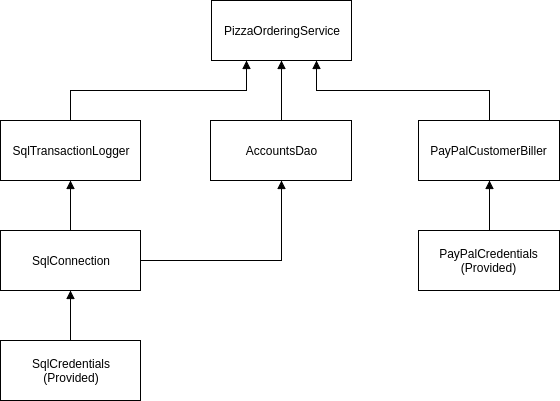
\includegraphics[width=0.7\textwidth]{renders/DependencyInjection.png}
      \caption{Dependency Graph built by Guice}
      \label{fig:depGraph}
\end{figure}

This leads to extremely simple code for the \java{PizzaOrderingService} in which the logic is entirely separated from the dependency management.

\lstinputlisting[
  caption={Pizza Ordering Service using Dependency Injection},
  label={lst:DI},
  style=javaStyle
  ]{code/technologies/DI.java}

Aside from abstracting away the dependency instantiation, dependency injection also has the added benefit in that all of a classes dependencies become part of the classes signature. There are no required dependencies that are buried within the implementation logic. This makes the code much simpler to test. The \java{PayPalCustomerBiller} used by the class is essentially hardwired into the code that does not use dependency injection (\refcode{lst:noDI}), meaning there is no way to test this class without actually billing a (fake) customer. However as the \java{PayPalCustomerBiller} used by the dependency injected code (\refcode{lst:DI}), a mock of this object (which skips the actual billing, but returns results as if it actually billed a customer) can be provided to the class and used for testing purposes.   

\subsection{Immutables - Immutability for Java}
Immutability is a programming paradigm in which once an object is created, it may never been changed. At first glance this sounds like a bad idea which will result in redundant object creation, but the positives strongly outweigh the negatives. The primary benefit of immutability is that the programmer is \textbf{guaranteed} that any object they hold a reference to, will never be changed. This concept is closely tied to the concept of writing \textit{pure} functions. These are functions which have no external side effects. That is, they take in arguments and return a value, but do not change the input arguments (or any other state contained in the program) in any way. 

These benefits are best highlighted through sample code. Consider the case of a simple website where each login attempt by a user should be logged to a database table in order to detect a hacker trying to crack a password by repeatedly trying to login as a user. For obvious reasons, this table should not store the user's password (in case of real login attempts), so this should be stripped before logging it to the database. An example \java{LoginRequest} is shown in \refcode{lst:loginRequest}. A \java{LoginAttemptLogger} class is written to handle logging these attempts to the database and is shown in \refcode{lst:loginAttemptLogger}. The \java{logLoginAttempt} method handles stripping the password from the \java{LoginRequest} and writing it to the database. 

\lstinputlisting[
  caption={An Example LoginRequest},
  label={lst:loginRequest},
  style=javaStyle
  ]{code/technologies/immutability/LoginRequest.java}

\lstinputlisting[
  caption={An Example LoginAttemptLogger Implementation},
  label={lst:loginAttemptLogger},
  style=javaStyle
  ]{code/technologies/immutability/LoginAttemptLogger.java}

However this style of code is a recipie for disaster. The \java{LoginRequest} is mutable and the \java{logLoginAttempt} method contains a side effect in that it sets the password of the \java{LoginRequest} to an empty string. Some perfectly reasonable client code is shown in \refcode{lst:clientLoginCode} in which the client logs the login request to the database and subsequently tries to log in. In this case, no user will ever be able to login as all of the passwords of the login requests are always mutated to be an empty string. Thus, having \java{LoginRequest} as a mutable object causes a critical bug that will not be caught until runtime.

\lstinputlisting[
  caption={Perfectly Reasonable Client Login Code},
  label={lst:clientLoginCode},
  style=javaStyle
  ]{code/technologies/immutability/ClientLogin.java}

The solution to this problem is to create a new \java{LoginRequest} without the user's password and log that to the database. This can be done inside of the client login code (defensive copying) before passing the \java{LoginReuqest} to the \java{logLoginAttempt}. However if mutators are provided, it is extremelty likely that they will be used somewhere in the code. Thus the best solution is simply to not provide them at all - make the object entirely immutable. This in turn requires some clunky code inside of the client login method (see \refcode{lst:clunkyImmutableClient}), but avoid the issue caused by the side effect of \java{logLoginAttempt}. 

\lstinputlisting[
  caption={Logically Correct Login Code with Extra Boilerplate},
  label={lst:clunkyImmutableClient},
  style=javaStyle
  ]{code/technologies/immutability/ImmutableClientLogin.java}

The Immutables \cite{immutablesJava} provides a framework for autogenerating fully immutable object implementations in Java. These implementations provide extremely useful functionality such as implementing builders and providing methods for updating the fields of an object in an immutable way. The immutable data structure is defined using an interface (annotated with \java{@Value.Immutable}) which contains the getter methods for each desired field of the object. A class which implements this interface in an immutable way is then auto generated by the framework and can is then used in place of the interface. An example of the interface used for \java{LoginRequest} is shown in \refcode{lst:immutableLibLoginRequest}.

\lstinputlisting[
  caption={Interface Used to Define LoginRequest using Immutables Framework},
  label={lst:immutableLibLoginRequest},
  style=javaStyle
  ]{code/technologies/immutability/ImmutableLibLoginRequest.java}

The implementation of this interface generated by the framework then provides a \java{withFieldName} method for each of the fields defined, allowing a new instance of the object with the updated fields to be obtained with a single method call as shown in \refcode{lst:loginAttemptLoggerWithImmutable}. This solves the problem of mutating the \java{LoginRequest} that the client holds a reference to and drastically simplifies working with immutable objects in Java. This framework is used exstensively at HubSpot and is a major contributor to the simplicity of writing code without bugs at the company.

\lstinputlisting[
  caption={The LoginAttemptLogger Method using the Immutables Framework},
  label={lst:loginAttemptLoggerWithImmutable},
  style=javaStyle
  ]{code/technologies/immutability/LoginAttemptLoggerImmutable.java}


\subsection{Kafka - Streaming Platform}
Kafka \cite{kafka} is a horiztonally scalable, fault tolerant, distributed streaming platform used to read and write streams of data in real time. It is an extremely high performance system and is used exstensively by the \team{} team as the primary data pipeline. Kafka runs on it's own cluster and stores streams of records inside categories known as Kafka \textit{topics}. Kafka provides two key APIs that are used at HubSpot - one for producing records to a given Kafka topic and one for consuming records from a specific Kafka topic. Kafka is used exstensively inside of the team's internal pipeline, but also as an interface between teams. For example, the teams responsible for building out and rendering the full HTML body of an email to be sent on behalf of a customer can produce this ready to be sent email to a specific kafka topic. Kafka consumers owned by the \team{} team are subscribed to this topic and thus pick up the records published to these topics and can perform the send of the email. This entirely decouples the work done by teams by simply requiring teams to put messages onto Kafka to be handled elsewhere. An obvious alternative to using Kafka would be to simply expose a REST endpoint in which the message is posted to. However simple HTTP would struggle to support the volume of requests (upwards of 25M emails per day) seen by the \team{} team. As mentioned, Kafka is horizontally scalable, meaning the number of nodes on the Kafka cluster can simply grow as the number of messages published to Kafka increases. Similarly on the consumer side, the number of deployed workers subscribed to a given topic can simply be increased in order to meet the increased number of records published to the topic.

Kafka also provides another layer of granularity - partitions. Each Kafka topic is segmented into a number of partitions. Each partition is (at any given time) owned by exactly one Kafka consumer, but each Kafka consumer may own multiple partitions. This leads to an interesting case when choosing the number of partitions to use for a given topic. Ideally, the number of partitions should be a highly composite number \cite {highlyCompositeNumbers}. These are numbers which are divisible by many other numbers, for example 24 which is divisible by 2, 3, 4, 6, 8 and 12. To illustrate why, consider the case where 9 partitions are used - the work load is only equally distributed if 1, 3 or 9 consumers are used. Thus if 3 consumers isn't enough, scaling to five consumers means four consumers will be consuming from two partitions and one will only be consuming from one partition. Using a highly composite number of partitions allows for more flexibility when choosing the number of consumers. Kafka can also handle rebalancing the workload, by redistributing the partitions when the number of consumers changes. 

When messages are produced to a Kafka topic, a decision must be made on which paritition to assign the message to. This can be done intelligently with load balancing in mind, or simply using a round robin. Partitions can also be replicated in order to provide fault tolerance.

An example of a Kafka topic with two consumers is shown in \reffig{fig:kafka}. 

\begin{figure}[H]
      \centering
      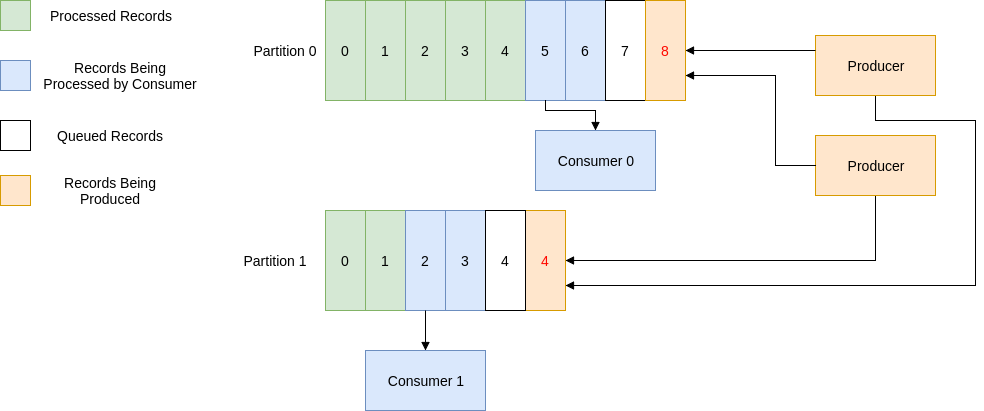
\includegraphics[width=\textwidth]{renders/Kafka.png}
      \caption{Kafka Producers and Consumers}
      \label{fig:kafka}
\end{figure}  

The current situation is outlined as follows:
\begin{itemize}
\item{Consumer 0 has successfully processed (and commited) messages 0 to 4 and is currently processing messages 5 and 6}
\item{Consumer 1 has successfully processed (and commited) messages 0 and 1 and is currently processing messages 2 and 3}
\item{Message 7 in partition 0 and message 4 in partition 1 have both been successfully produced and commited to the log}
\item{Message 8 in partition 1 and message 4 in parition two will be the next messages produced by the producers.}
\end{itemize}

Each message published to a Kafka partition gets an incremental id known as an \textit{offset}. Consumers are responsible for managing their offset in the message stream. Thus consumers can be configured to start from any offset, which can even allow for reprocessing of data should the need arise. This has been useful in the past at HubSpot when a bug has caused emails to fail to send. The consumers can have their offsets reset to when the bug first surfaced and the emails will be resent. However this is a delicate process and is only used as a last resort. The offsets for consumers 1 and 2 in \reffig{fig:kafka} would be 4 and 1 respectively.

An key concept to understand about Kafka is that consumers are presented with batches of records, of a configurable size. The batch size in \reffig{fig:kafka} is two. The records inside the batch may be processed out of order, but the batch of records is considered completed \textbf{only when every record in the batch has been processed}. In Kafka, only an entire batch of messages can be marked as processed. For example consider consumer 0 in \reffig{fig:kafka}. Should the consumer succeed to process message two, but fail to process message three, Kafka must be notified of the failure to process the batch of messages (or will notice a timeout) and the entire batch will be retried.


Another interesting concept in Kafka is consumer groups. Consider the case where two entirely separate sets of workers (running different code) need to read from the same Kafka topic. Both sets of workers should be able to process every message that is published to the Kafka and this is what consumer groups provides. Without consumer groups, another worker could be set up in order to read from the Kafka topic, but as discussed, it would only acquire a certain number of partitions and thus miss some messages (and steal messages from existing workers). The solution is to specify the consumer group that each running worker belongs to. In this case, since there are two sets of workers, both doing different things, there should be two consumer groups. Kafka will then treat all of the consumers in each consumer group as if there are no other sets of workers reading from the Kafka topic. This feature is best understood by considering the two edge cases:

\begin{itemize}
\item{If all workers are in the \textit{same} consumer group, Kafka simply load balances the partitions across the number of workers}
\item{If all workers are in \textit{different} consumer groups, each worker will have its own offset in \textbf{all} of the partitions. That is, the worker responsible for partition zero in consumer group A may have a current offset of 100, while the worker responsible for partition zero in consumer group B may have a current offset of 0. This is essentially, publish-subscribe (pub-sub) behaviour. All of the workers will simply see all of the events and the rate of consumption of a certain worker has no impact on the rate of consumption of another worker.}
\end{itemize}

Continuing with the previous example (of having all of the emails to be sent through HubSpot contained on a Kafka topic), the following consumer groups could be set up in order to both send every email that appears on the topic and to bill each customer for each email that appears on the topic. This is also shown in \reffig{fig:consumerGroups}
\begin{labeling}{SENDING}
\item[SENDING]{This consumer group would contain all of the \team{} team's consumers. There would likely be a lot of consumer's in this consumer group in order to keep up with the time consuming process of actually sending the emails on behalf of the customers. These would be time critical and thus performance and efficiency would be critical. The delta between the current offset (the index of the most recently produced message) and the oldest offset (the index of the oldest message still being processed) for each partition would likely be carefully monitored to ensure the consumers are not falling behind}
\item[BILLING]{This consumer group would perhaps simply read the account number of the customer sending the email and bill that customer. This consumer group would be considerably less time critical and would likely only need to perform some light weight task for each message on the Kafka topic.}
\end{labeling}


\begin{figure}[H]
      \centering
      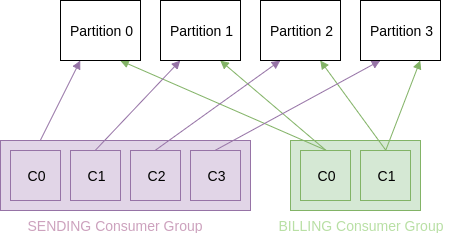
\includegraphics[width=0.6\textwidth]{renders/ConsumerGroups.png}
      \caption{Partition Assignments with Multiple Consumer Groups}
      \label{fig:consumerGroups}
\end{figure}  

A final note of interest regarding Kafka is that it provides and \textit{at-least-once} guarantee that messages will arive at consumers for processing. If a single message in a batch of messages cannot be processed for whatever reason, the entire batch will be retried. Thus external idempotency logic is required in order to obtain an \textit{exactly-once} processing guarantee. The \team{} team uses a simple HBase table in order to lock each email that is to be sent, prior to actually sending it. 

% \subsection{MySql}
% Indexes, liquibase, InnoDB

% \subsection{HBase}

% \subsection{ZooKeeper (Circus)}\

% \subsection{Maven - Dependency Management}

\subsection{Hadoop}

\subsection{gRPC and Protobuf}



\section{Email Specific Technologies}
\subsection{DNS} \label{sec:DNS}
Although not entirely email specific, DNS is extremely critical for the \team{} team. Aside from teams working on the HubSpot platform, most other teams need not concern themselves with DNS at all. 

DIAGRAM OF RECORDS?
DKIM SELECTORS **
each of the record types, when an email arrives what is looked at, look at the tld, then zones on that tld then record types and key values etc. UDP typically, fallback to TCP
\subsection{SMTP} \label{sec:smtp}

\section{System Management and Health Monitoring}
While working on projects of this magnitude, bugs and issues are an inevitability. The amount of traffic seen by these systems compounds any small issues or bugs present in the system. As such, it is critcal to have systems in place which monitor the health of the system and inform the team of any potential issues with the system. Whatsmore, these issues must be continuously examined and remedial action must be taken where applicable. The \team{} team made use of several tools and methods for monitoring the health of their systems, a subset of which are outlined below:

\subsection{Log4j2}
Log4j2 \cite{log4j2} is a Java framework which is provides facilities for logging to different log levels and advanced log filtering (for example with regular expressions). This provides an excellent facility for understanding why systems are behaving unexpectedly in production. A common pattern is to insert log messages to a low priority log level (eg DEBUG) which describe the state of the system or the code path taken. Typically when the system is behaving normally, a highger priortiy log level is set (eg INFO) meaning these finer grained log messages are skipped. However, should an issue arise, the log level can then be easily switched to the lower priority temporarily to get a more detailed insight into why the system is misbehaving. This pattern allows detailed log messages to be produced only when they are needed, reducing the amount of noise present in the logs. The framework also provides the ERROR debug mode which can log error messages as uncaught exceptions without killing the currently executing thread.

\subsection{Sentry}
Sentry \cite{sentry} is an online platform which logs uncaught exceptions that arise during program execution. This greatly simplifies the task of finding out the reason for a system fault or failure without the need to trawl through pages of log files. Sentry logs the full stack trace associated with an exception, the time of occuence and other pieces of meta data such as the name of the deployable. It uses this data to monitor the occurences of particular exceptions over time, provides facilities for opening and closing GitHub issues and most importantly, to send an email to all those subscribed to the project (eg the \team{} in this case) when an exception occurs. Sentry proves to be extremely useful at deploy time. Obviously when deploying new code to production servers, one must be sure that the changes did not cause the system to enter an unhealthy state. Provided the code is well written and that unexpected exceptions that occur are not silently swallowed, Sentry can be monitored at deploy time in order to help provide the engineer with confidence that the deployed changes were non breaking. Sentry also provides support for integrating into the aforementioned Log4j2. Sentry can monitor ERROR level log messages that are produced by Log4j2 and subsequently log these error messages to sentry. As an engineer this combination of tools is extremely useful for indicating that the system has found an issue, without killing the thread. This is ideal in cases where some work has been done and the system has encountered a critical error, but does not need to be restarted. This mitigates the need to repeat the work, but still enforms the team that an error has occured by logging an exception to Sentry.

\subsection{SignalFX}
SignalFX \cite{sigfx} is a online tool for recording metrics and data visualization. Gathering and analysing metrics is a key part of ensuring the health of a comlpex system. When things start to fail, SignalFX is the first place engineers look to. SignalFX essentially allows data to be dumped to the cloud and for complex graphs and charts to be rendered in real time using this data. SignalFX supports creating dashboards consiting of many of these graphs and charts. The \team{} team has several of these dashboards, each encapsulating a single part of the system. When problems inevitably arise, the team can examine these dashboards in order to try and isolate and find the problem. Once remedial action has been taken, the dashboards can be monitored to ensure the desired effect takes place. Being able to see these metrics in close to real time is incredibily useful for diagnosing faults with the system. It also serves as an excellent mechanism for finding parts of the system that can be improved. For example, critical code paths can be timed and the results logged to sentry. This allows accurate inferences to be made about parts of the system and allows the team to target these parts.

SignalFX also allows for detectors to be configured. For example, a chart could be created monitoring the number of emails sent in the past minute by each IP address responsible for sending emails. A detector can then be put in place to detect if this number falls below a certain threshold. Detectors can be configured to alert via email and slack when they fire, allowing engineers to be notified. 

SignalFX also supports complex data aggregations. This is beneficial as it decouples calculations that need to be done on metrics from the code which the metrics are monitoring. Perform any sort of data manipulation in performance critical code paths is obviously not desirable when every millisecond counts. Instead, metrics gathering is as simple as producing the data to SignalFX. The complex graphs and charts can then be configured inside of the SignalFX tool, entirely independant to the production code. 